\documentclass[crop=false,class=book]{standalone}
%---------------PREAMBLE------------%
%---------------------------Packages----------------------------%
\usepackage{geometry}
\geometry{b5paper, margin=1.0in}
\usepackage[T1]{fontenc}
\usepackage{graphicx, float}            % Graphics/Images.
\usepackage{natbib}                     % For bibliographies.
\bibliographystyle{agsm}                % Bibliography style.
\usepackage[french, english]{babel}     % Language typesetting.
\usepackage[dvipsnames]{xcolor}         % Color names.
\usepackage{listings}                   % Verbatim-Like Tools.
\usepackage{mathtools, esint, mathrsfs} % amsmath and integrals.
\usepackage{amsthm, amsfonts, amssymb}  % Fonts and theorems.
\usepackage{tcolorbox}                  % Frames around theorems.
\usepackage{upgreek}                    % Non-Italic Greek.
\usepackage{fmtcount, etoolbox}         % For the \book{} command.
\usepackage[newparttoc]{titlesec}       % Formatting chapter, etc.
\usepackage{titletoc}                   % Allows \book in toc.
\usepackage[nottoc]{tocbibind}          % Bibliography in toc.
\usepackage[titles]{tocloft}            % ToC formatting.
\usepackage{pgfplots, tikz}             % Drawing/graphing tools.
\usepackage{imakeidx}                   % Used for index.
\usetikzlibrary{
    calc,                   % Calculating right angles and more.
    angles,                 % Drawing angles within triangles.
    arrows.meta,            % Latex and Stealth arrows.
    quotes,                 % Adding labels to angles.
    positioning,            % Relative positioning of nodes.
    decorations.markings,   % Adding arrows in the middle of a line.
    patterns,
    arrows
}                                       % Libraries for tikz.
\pgfplotsset{compat=1.9}                % Version of pgfplots.
\usepackage[font=scriptsize,
            labelformat=simple,
            labelsep=colon]{subcaption} % Subfigure captions.
\usepackage[font={scriptsize},
            hypcap=true,
            labelsep=colon]{caption}    % Figure captions.
\usepackage[pdftex,
            pdfauthor={Ryan Maguire},
            pdftitle={Mathematics and Physics},
            pdfsubject={Mathematics, Physics, Science},
            pdfkeywords={Mathematics, Physics, Computer Science, Biology},
            pdfproducer={LaTeX},
            pdfcreator={pdflatex}]{hyperref}
\hypersetup{
    colorlinks=true,
    linkcolor=blue,
    filecolor=magenta,
    urlcolor=Cerulean,
    citecolor=SkyBlue
}                           % Colors for hyperref.
\usepackage[toc,acronym,nogroupskip,nopostdot]{glossaries}
\usepackage{glossary-mcols}
%------------------------Theorem Styles-------------------------%
\theoremstyle{plain}
\newtheorem{theorem}{Theorem}[section]

% Define theorem style for default spacing and normal font.
\newtheoremstyle{normal}
    {\topsep}               % Amount of space above the theorem.
    {\topsep}               % Amount of space below the theorem.
    {}                      % Font used for body of theorem.
    {}                      % Measure of space to indent.
    {\bfseries}             % Font of the header of the theorem.
    {}                      % Punctuation between head and body.
    {.5em}                  % Space after theorem head.
    {}

% Italic header environment.
\newtheoremstyle{thmit}{\topsep}{\topsep}{}{}{\itshape}{}{0.5em}{}

% Define environments with italic headers.
\theoremstyle{thmit}
\newtheorem*{solution}{Solution}

% Define default environments.
\theoremstyle{normal}
\newtheorem{example}{Example}[section]
\newtheorem{definition}{Definition}[section]
\newtheorem{problem}{Problem}[section]

% Define framed environment.
\tcbuselibrary{most}
\newtcbtheorem[use counter*=theorem]{ftheorem}{Theorem}{%
    before=\par\vspace{2ex},
    boxsep=0.5\topsep,
    after=\par\vspace{2ex},
    colback=green!5,
    colframe=green!35!black,
    fonttitle=\bfseries\upshape%
}{thm}

\newtcbtheorem[auto counter, number within=section]{faxiom}{Axiom}{%
    before=\par\vspace{2ex},
    boxsep=0.5\topsep,
    after=\par\vspace{2ex},
    colback=Apricot!5,
    colframe=Apricot!35!black,
    fonttitle=\bfseries\upshape%
}{ax}

\newtcbtheorem[use counter*=definition]{fdefinition}{Definition}{%
    before=\par\vspace{2ex},
    boxsep=0.5\topsep,
    after=\par\vspace{2ex},
    colback=blue!5!white,
    colframe=blue!75!black,
    fonttitle=\bfseries\upshape%
}{def}

\newtcbtheorem[use counter*=example]{fexample}{Example}{%
    before=\par\vspace{2ex},
    boxsep=0.5\topsep,
    after=\par\vspace{2ex},
    colback=red!5!white,
    colframe=red!75!black,
    fonttitle=\bfseries\upshape%
}{ex}

\newtcbtheorem[auto counter, number within=section]{fnotation}{Notation}{%
    before=\par\vspace{2ex},
    boxsep=0.5\topsep,
    after=\par\vspace{2ex},
    colback=SeaGreen!5!white,
    colframe=SeaGreen!75!black,
    fonttitle=\bfseries\upshape%
}{not}

\newtcbtheorem[use counter*=remark]{fremark}{Remark}{%
    fonttitle=\bfseries\upshape,
    colback=Goldenrod!5!white,
    colframe=Goldenrod!75!black}{ex}

\newenvironment{bproof}{\textit{Proof.}}{\hfill$\square$}
\tcolorboxenvironment{bproof}{%
    blanker,
    breakable,
    left=3mm,
    before skip=5pt,
    after skip=10pt,
    borderline west={0.6mm}{0pt}{green!80!black}
}

\AtEndEnvironment{lexample}{$\hfill\textcolor{red}{\blacksquare}$}
\newtcbtheorem[use counter*=example]{lexample}{Example}{%
    empty,
    title={Example~\theexample},
    boxed title style={%
        empty,
        size=minimal,
        toprule=2pt,
        top=0.5\topsep,
    },
    coltitle=red,
    fonttitle=\bfseries,
    parbox=false,
    boxsep=0pt,
    before=\par\vspace{2ex},
    left=0pt,
    right=0pt,
    top=3ex,
    bottom=1ex,
    before=\par\vspace{2ex},
    after=\par\vspace{2ex},
    breakable,
    pad at break*=0mm,
    vfill before first,
    overlay unbroken={%
        \draw[red, line width=2pt]
            ([yshift=-1.2ex]title.south-|frame.west) to
            ([yshift=-1.2ex]title.south-|frame.east);
        },
    overlay first={%
        \draw[red, line width=2pt]
            ([yshift=-1.2ex]title.south-|frame.west) to
            ([yshift=-1.2ex]title.south-|frame.east);
    },
}{ex}

\AtEndEnvironment{ldefinition}{$\hfill\textcolor{Blue}{\blacksquare}$}
\newtcbtheorem[use counter*=definition]{ldefinition}{Definition}{%
    empty,
    title={Definition~\thedefinition:~{#1}},
    boxed title style={%
        empty,
        size=minimal,
        toprule=2pt,
        top=0.5\topsep,
    },
    coltitle=Blue,
    fonttitle=\bfseries,
    parbox=false,
    boxsep=0pt,
    before=\par\vspace{2ex},
    left=0pt,
    right=0pt,
    top=3ex,
    bottom=0pt,
    before=\par\vspace{2ex},
    after=\par\vspace{1ex},
    breakable,
    pad at break*=0mm,
    vfill before first,
    overlay unbroken={%
        \draw[Blue, line width=2pt]
            ([yshift=-1.2ex]title.south-|frame.west) to
            ([yshift=-1.2ex]title.south-|frame.east);
        },
    overlay first={%
        \draw[Blue, line width=2pt]
            ([yshift=-1.2ex]title.south-|frame.west) to
            ([yshift=-1.2ex]title.south-|frame.east);
    },
}{def}

\AtEndEnvironment{ltheorem}{$\hfill\textcolor{Green}{\blacksquare}$}
\newtcbtheorem[use counter*=theorem]{ltheorem}{Theorem}{%
    empty,
    title={Theorem~\thetheorem:~{#1}},
    boxed title style={%
        empty,
        size=minimal,
        toprule=2pt,
        top=0.5\topsep,
    },
    coltitle=Green,
    fonttitle=\bfseries,
    parbox=false,
    boxsep=0pt,
    before=\par\vspace{2ex},
    left=0pt,
    right=0pt,
    top=3ex,
    bottom=-1.5ex,
    breakable,
    pad at break*=0mm,
    vfill before first,
    overlay unbroken={%
        \draw[Green, line width=2pt]
            ([yshift=-1.2ex]title.south-|frame.west) to
            ([yshift=-1.2ex]title.south-|frame.east);},
    overlay first={%
        \draw[Green, line width=2pt]
            ([yshift=-1.2ex]title.south-|frame.west) to
            ([yshift=-1.2ex]title.south-|frame.east);
    }
}{thm}

%--------------------Declared Math Operators--------------------%
\DeclareMathOperator{\adjoint}{adj}         % Adjoint.
\DeclareMathOperator{\Card}{Card}           % Cardinality.
\DeclareMathOperator{\curl}{curl}           % Curl.
\DeclareMathOperator{\diam}{diam}           % Diameter.
\DeclareMathOperator{\dist}{dist}           % Distance.
\DeclareMathOperator{\Div}{div}             % Divergence.
\DeclareMathOperator{\Erf}{Erf}             % Error Function.
\DeclareMathOperator{\Erfc}{Erfc}           % Complementary Error Function.
\DeclareMathOperator{\Ext}{Ext}             % Exterior.
\DeclareMathOperator{\GCD}{GCD}             % Greatest common denominator.
\DeclareMathOperator{\grad}{grad}           % Gradient
\DeclareMathOperator{\Ima}{Im}              % Image.
\DeclareMathOperator{\Int}{Int}             % Interior.
\DeclareMathOperator{\LC}{LC}               % Leading coefficient.
\DeclareMathOperator{\LCM}{LCM}             % Least common multiple.
\DeclareMathOperator{\LM}{LM}               % Leading monomial.
\DeclareMathOperator{\LT}{LT}               % Leading term.
\DeclareMathOperator{\Mod}{mod}             % Modulus.
\DeclareMathOperator{\Mon}{Mon}             % Monomial.
\DeclareMathOperator{\multideg}{mutlideg}   % Multi-Degree (Graphs).
\DeclareMathOperator{\nul}{nul}             % Null space of operator.
\DeclareMathOperator{\Ord}{Ord}             % Ordinal of ordered set.
\DeclareMathOperator{\Prin}{Prin}           % Principal value.
\DeclareMathOperator{\proj}{proj}           % Projection.
\DeclareMathOperator{\Refl}{Refl}           % Reflection operator.
\DeclareMathOperator{\rk}{rk}               % Rank of operator.
\DeclareMathOperator{\sgn}{sgn}             % Sign of a number.
\DeclareMathOperator{\sinc}{sinc}           % Sinc function.
\DeclareMathOperator{\Span}{Span}           % Span of a set.
\DeclareMathOperator{\Spec}{Spec}           % Spectrum.
\DeclareMathOperator{\supp}{supp}           % Support
\DeclareMathOperator{\Tr}{Tr}               % Trace of matrix.
%--------------------Declared Math Symbols--------------------%
\DeclareMathSymbol{\minus}{\mathbin}{AMSa}{"39} % Unary minus sign.
%------------------------New Commands---------------------------%
\DeclarePairedDelimiter\norm{\lVert}{\rVert}
\DeclarePairedDelimiter\ceil{\lceil}{\rceil}
\DeclarePairedDelimiter\floor{\lfloor}{\rfloor}
\newcommand*\diff{\mathop{}\!\mathrm{d}}
\newcommand*\Diff[1]{\mathop{}\!\mathrm{d^#1}}
\renewcommand*{\glstextformat}[1]{\textcolor{RoyalBlue}{#1}}
\renewcommand{\glsnamefont}[1]{\textbf{#1}}
\renewcommand\labelitemii{$\circ$}
\renewcommand\thesubfigure{%
    \arabic{chapter}.\arabic{figure}.\arabic{subfigure}}
\addto\captionsenglish{\renewcommand{\figurename}{Fig.}}
\numberwithin{equation}{section}

\renewcommand{\vector}[1]{\boldsymbol{\mathrm{#1}}}

\newcommand{\uvector}[1]{\boldsymbol{\hat{\mathrm{#1}}}}
\newcommand{\topspace}[2][]{(#2,\tau_{#1})}
\newcommand{\measurespace}[2][]{(#2,\varSigma_{#1},\mu_{#1})}
\newcommand{\measurablespace}[2][]{(#2,\varSigma_{#1})}
\newcommand{\manifold}[2][]{(#2,\tau_{#1},\mathcal{A}_{#1})}
\newcommand{\tanspace}[2]{T_{#1}{#2}}
\newcommand{\cotanspace}[2]{T_{#1}^{*}{#2}}
\newcommand{\Ckspace}[3][\mathbb{R}]{C^{#2}(#3,#1)}
\newcommand{\funcspace}[2][\mathbb{R}]{\mathcal{F}(#2,#1)}
\newcommand{\smoothvecf}[1]{\mathfrak{X}(#1)}
\newcommand{\smoothonef}[1]{\mathfrak{X}^{*}(#1)}
\newcommand{\bracket}[2]{[#1,#2]}

%------------------------Book Command---------------------------%
\makeatletter
\renewcommand\@pnumwidth{1cm}
\newcounter{book}
\renewcommand\thebook{\@Roman\c@book}
\newcommand\book{%
    \if@openright
        \cleardoublepage
    \else
        \clearpage
    \fi
    \thispagestyle{plain}%
    \if@twocolumn
        \onecolumn
        \@tempswatrue
    \else
        \@tempswafalse
    \fi
    \null\vfil
    \secdef\@book\@sbook
}
\def\@book[#1]#2{%
    \refstepcounter{book}
    \addcontentsline{toc}{book}{\bookname\ \thebook:\hspace{1em}#1}
    \markboth{}{}
    {\centering
     \interlinepenalty\@M
     \normalfont
     \huge\bfseries\bookname\nobreakspace\thebook
     \par
     \vskip 20\p@
     \Huge\bfseries#2\par}%
    \@endbook}
\def\@sbook#1{%
    {\centering
     \interlinepenalty \@M
     \normalfont
     \Huge\bfseries#1\par}%
    \@endbook}
\def\@endbook{
    \vfil\newpage
        \if@twoside
            \if@openright
                \null
                \thispagestyle{empty}%
                \newpage
            \fi
        \fi
        \if@tempswa
            \twocolumn
        \fi
}
\newcommand*\l@book[2]{%
    \ifnum\c@tocdepth >-3\relax
        \addpenalty{-\@highpenalty}%
        \addvspace{2.25em\@plus\p@}%
        \setlength\@tempdima{3em}%
        \begingroup
            \parindent\z@\rightskip\@pnumwidth
            \parfillskip -\@pnumwidth
            {
                \leavevmode
                \Large\bfseries#1\hfill\hb@xt@\@pnumwidth{\hss#2}
            }
            \par
            \nobreak
            \global\@nobreaktrue
            \everypar{\global\@nobreakfalse\everypar{}}%
        \endgroup
    \fi}
\newcommand\bookname{Book}
\renewcommand{\thebook}{\texorpdfstring{\Numberstring{book}}{book}}
\providecommand*{\toclevel@book}{-2}
\makeatother
\titleformat{\part}[display]
    {\Large\bfseries}
    {\partname\nobreakspace\thepart}
    {0mm}
    {\Huge\bfseries}
\titlecontents{part}[0pt]
    {\large\bfseries}
    {\partname\ \thecontentslabel: \quad}
    {}
    {\hfill\contentspage}
\titlecontents{chapter}[0pt]
    {\bfseries}
    {\chaptername\ \thecontentslabel:\quad}
    {}
    {\hfill\contentspage}
\newglossarystyle{longpara}{%
    \setglossarystyle{long}%
    \renewenvironment{theglossary}{%
        \begin{longtable}[l]{{p{0.25\hsize}p{0.65\hsize}}}
    }{\end{longtable}}%
    \renewcommand{\glossentry}[2]{%
        \glstarget{##1}{\glossentryname{##1}}%
        &\glossentrydesc{##1}{~##2.}
        \tabularnewline%
        \tabularnewline
    }%
}
\newglossary[not-glg]{notation}{not-gls}{not-glo}{Notation}
\newcommand*{\newnotation}[4][]{%
    \newglossaryentry{#2}{type=notation, name={\textbf{#3}, },
                          text={#4}, description={#4},#1}%
}
%--------------------------LENGTHS------------------------------%
% Spacings for the Table of Contents.
\addtolength{\cftsecnumwidth}{1ex}
\addtolength{\cftsubsecindent}{1ex}
\addtolength{\cftsubsecnumwidth}{1ex}
\addtolength{\cftfignumwidth}{1ex}
\addtolength{\cfttabnumwidth}{1ex}

% Indent and paragraph spacing.
\setlength{\parindent}{0em}
\setlength{\parskip}{0em}
%---------------GLOSSARY------------%
\makeglossaries
\loadglsentries{../../glossary}
\loadglsentries{../../acronym}
%--------------Title Page-----------%
\begin{document}
\chapter{Easy Data Example}
\section{Example 1}
\begin{center}
    \LARGE{RSS\_2005\_123\_ X43\_ E \par
    Rev7-E Cassini Radio Science Ring Occultation: Geometry, Data Calibration, and Reconstructed Optical Depth and Phase Shift Profiles at 1 and 10km Resolution \par
    November 28, 2017\par}
\end{center}
\begin{figure}[H]
    \centering
    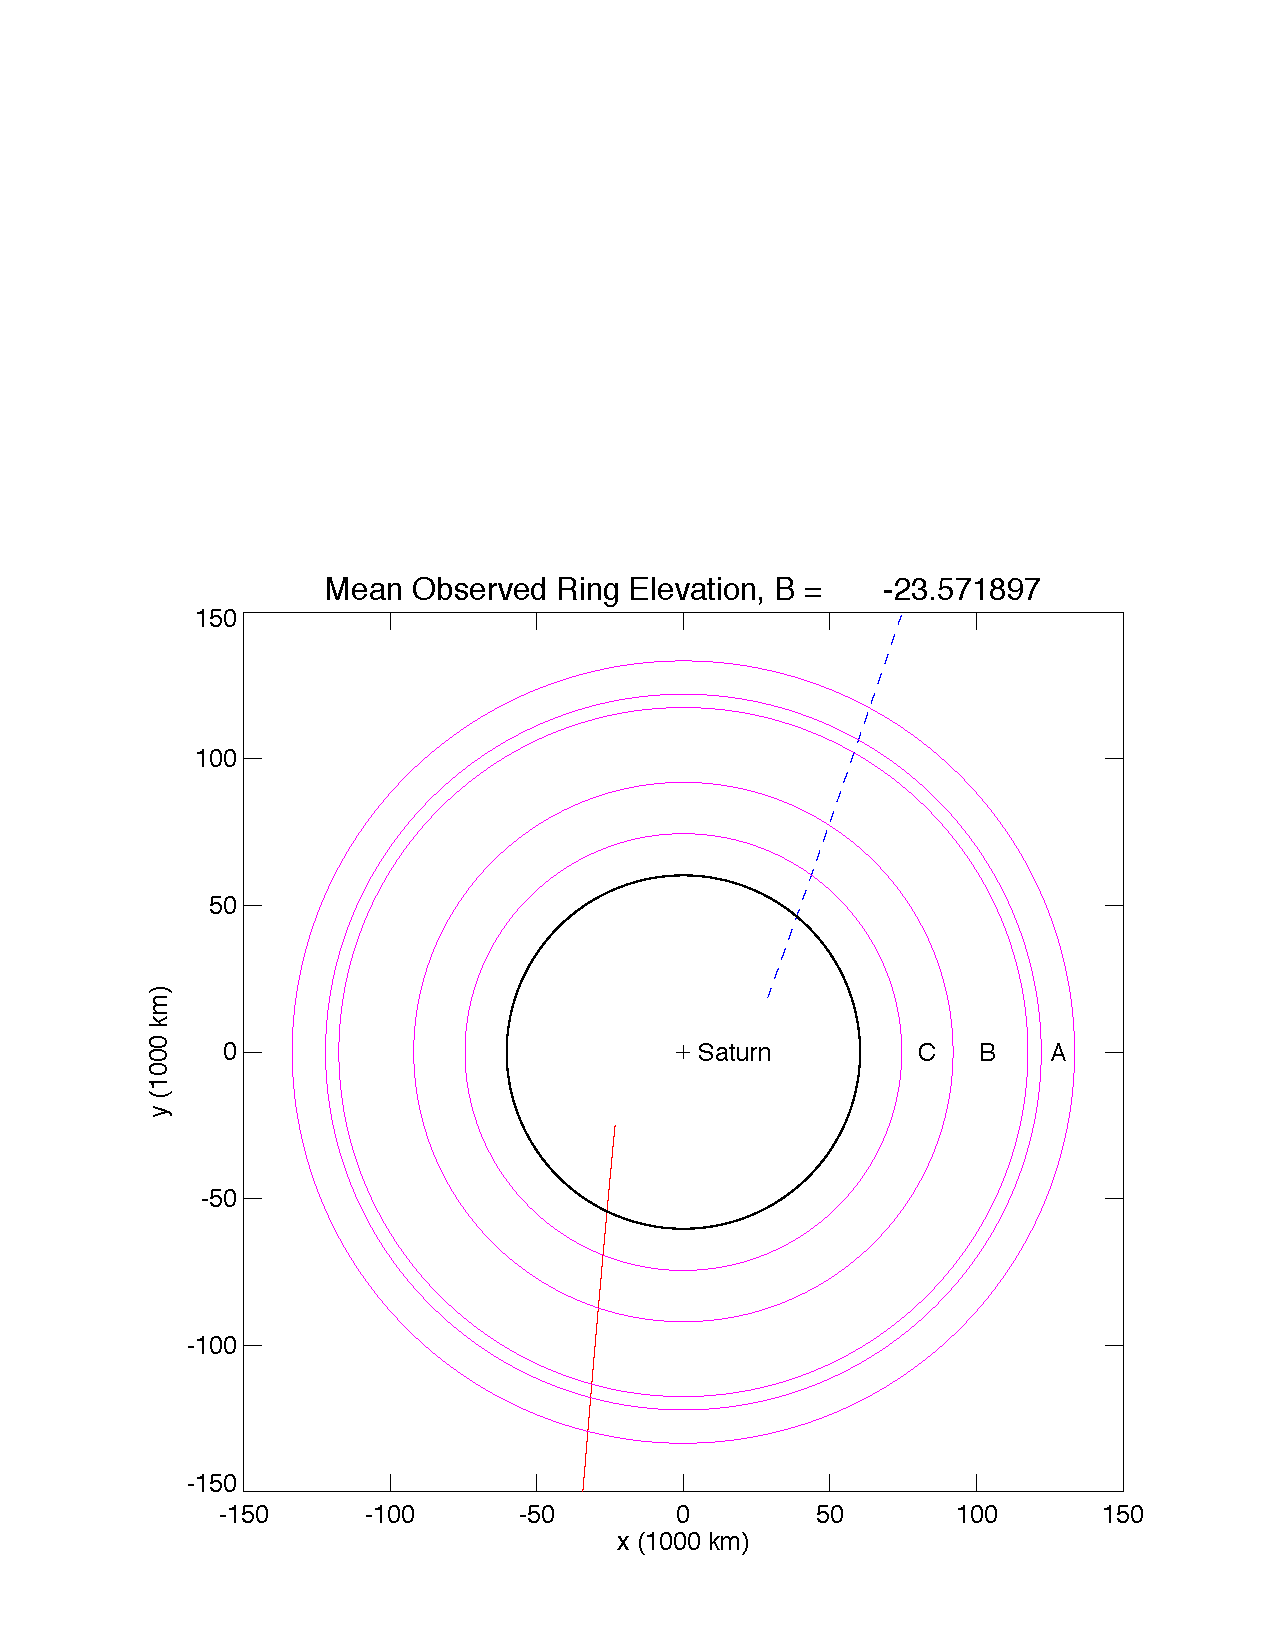
\includegraphics[page=1,trim = {0.67in 0.5in 0.5in 3.1in},clip,width=\textwidth]{Rev007_E_X43_summary_p1_08FEB2018.pdf}
    \caption*{The radio occultation track as seen looking down on the ring plane. The solid red track is relative to a reference direction defined by the direction to Earth, The dashed blue track is relative to a reference direction defined by the ascending node of J2000 on the ring plane.}
\end{figure}
\begin{table}[H]
    \centering
    \begin{tabular}{l l} 
        \hline
        Symbol 			& Parameter Name \\ % [0.5ex] 
        \hline
        $t_{OET}$		& OBSERVED EVENT TIME \\ 
        $t_{RET}$ 		& RING EVENT TIME \\
        $t_{SET}$ 		& SPACECRAFT EVENT TIME \\
        $\rho$	 		& RING RADIUS \\
        $\phi_{RL}$		& RING LONGITUDE \\
        $\phi_{ORA}$	& OBSERVED RING AZIMUTH \\
        $B$				& OBSERVED RING ELEVATION \\
        $D$				& SPACECRAFT TO RING INTERCEPT DISTANCE \\
        $\partial\rho/\partial t$	& RING INTERCEPT RADIAL VELOCITY \\
        $\partial\theta/\partial t$	& RING INTERCEPT AZIMUTHAL VELOCITY \\
        $F$				& FRESNEL SCALE \\
        $R_{impact}$	& IMPACT RADIUS \\
        $r_x$			& SPACECRAFT POSITION X \\
        $r_y$			& SPACECRAFT POSITION Y \\
        $r_z$			& SPACECRAFT POSITIION Z \\
        $v_x$			& SPACECRAFT VELOCITY X \\
        $v_y$			& SPACECRAFT VELOCITY Y \\
        $v_z$			& SPACECRAFT VELOCITY Z \\
        \hline
    \end{tabular}
    \caption[Easy Data Parameters for Geo File]{Glossary of parameters in file RSS\_2005\_123\_ X43\_ E\_ GEO.TAB. See companion label (.LBL) file for description of parameters.}
    \label{tab:easy_data_glossary_of_parameters_in_file_rss_2005_123_x43_e_geo_tab}
\end{table}
\begin{table}[H]
    \centering
    \begin{tabular}{l l}
        \hline
        Symbol			& Parameter Name \\
        \hline
        $t_{OET}$		& OBSERVED EVENT TIME \\
        $f_{sky}$		& SKY FREQUENCY \\
        $f_{resid}$		& RESIDUAL FREQUENCY \\
        $P_{free}$		& FREESPACE POWER \\
        \hline
    \end{tabular}
    \caption[Easy Data Parameters for Cal File]{Glossary of calibration data in file RSS\_2005\_123\_ X43\_ E\_ CAL.TAB. See companion label (.LBL) file for description of the data.}
    \label{tab:easy_data_table_glossary_of_calibration_data_in_file_RSS_2005_123_x45_e_cal_tab}
\end{table}
\begin{table}[H]
    \centering
    \begin{tabular}{l l}
        \hline
        Symbol			& Parameter Name \\
        \hline
        $\rho$			& RING RADIUS \\
        $\Delta\rho$		& RADIUS CORRECTION \\
        $\phi_{RL}$		& RING LONGITUDE \\
        $\phi_{ORA}$		& OBSERVED RING AZIMUTH \\
        $\tau$			& NORMAL OPTICAL DEPTH \\
        $\phi$			& PHASE SHIFT \\
        $\tau_{TH}$		& NORMAL OPTICAL DEPTH THRESHOLD \\
        $t_{OET}$			& OBSERVED EVENT TIME \\
        $t_{RET}$			& RING EVENT TIME \\
        $t_{SET}$			& SPACECRAFT EVENT TIME \\
        $B$				& OBSERVED RING ELEVATION \\
        \hline
    \end{tabular}
    \caption[Easy Data Parameters for Tau File]{Glossary of optical depth, phase shift, and selected geometry parameters contained in the files RSS\_2005\_123\_X43\_E\_TAU\_01KM.TAB and RSS\_2005\_123\_X43\_E\_TAU\_10KM.TAB. See companion label (.LBL) files for description of the data.}
\end{table}
\begin{figure}[H]
	    \centering
        \includegraphics[page=2,trim = {0.8in 0.5in 0.21in 0.45in},clip,width=\textwidth]{Rev007_E_X43_summary_p1_08FEB2018.pdf}
	        \caption[Occultation Geometry]{Occultation geometry parameters in file Rev007\_E\_ X43\_GEO.tab}
	        \label{fig:easy_dqata_fig_occultation_geo_parameters_inf_file_rev007_E_X43_geo_tab}
\end{figure}
\begin{figure}[H]
        \includegraphics[page=3,trim = {0.8in 0.5in 0.21in 0.45in},clip,width=\textwidth]{Rev007_E_X43_summary_p1_08FEB2018.pdf}
	        \caption[More Occultation Geometry]{See caption of \ref{fig:easy_dqata_fig_occultation_geo_parameters_inf_file_rev007_E_X43_geo_tab}.}
	\end{figure}
\begin{figure}[H]
    \centering
    \includegraphics[page=4,trim = {0.67in 0.5in 0.45in 0.5in},clip,width=\textwidth]{Rev007_E_X43_summary_p1_08FEB2018.pdf}
	    \caption[Calibration Data contained in the Easy Data]{Calibration data in file Rev007\_E\_X43\_CAL.TAB. The frequency residuals data (the smooth curve, in the second panel) is used to steer the carrier signal to the middle of the recording bandwidth. The free-space power data (the smooth curve in the third panel) is used to normalize signal power measurements so that the corresponding optical depth has nearly zero value in the absence of rings. Least-square fitting techniques to frequency and power estimates of the direct signal (the green curves in the second and third panels, respectively) are used to compute the calibration data.}
\end{figure}
\begin{figure}[H]
    \centering
    \includegraphics[page=5,trim = {0.8in 0.5in 0.21in 0.45in},clip,width=\textwidth]{Rev007_E_X43_summary_p1_08FEB2018.pdf}
	\caption[Even More Occultation Geometry]{Ring radius correction and selected occultation geometry parameters contained in the files RSS\_2005\_123\_X43\_E\_TAU\_01KM.TAB (green) and RSS\_2005\_123\_X43\_E\_TAU\_10KM.TAB (blue).}
\end{figure}
\clearpage
\begin{figure}[H]
    \centering
    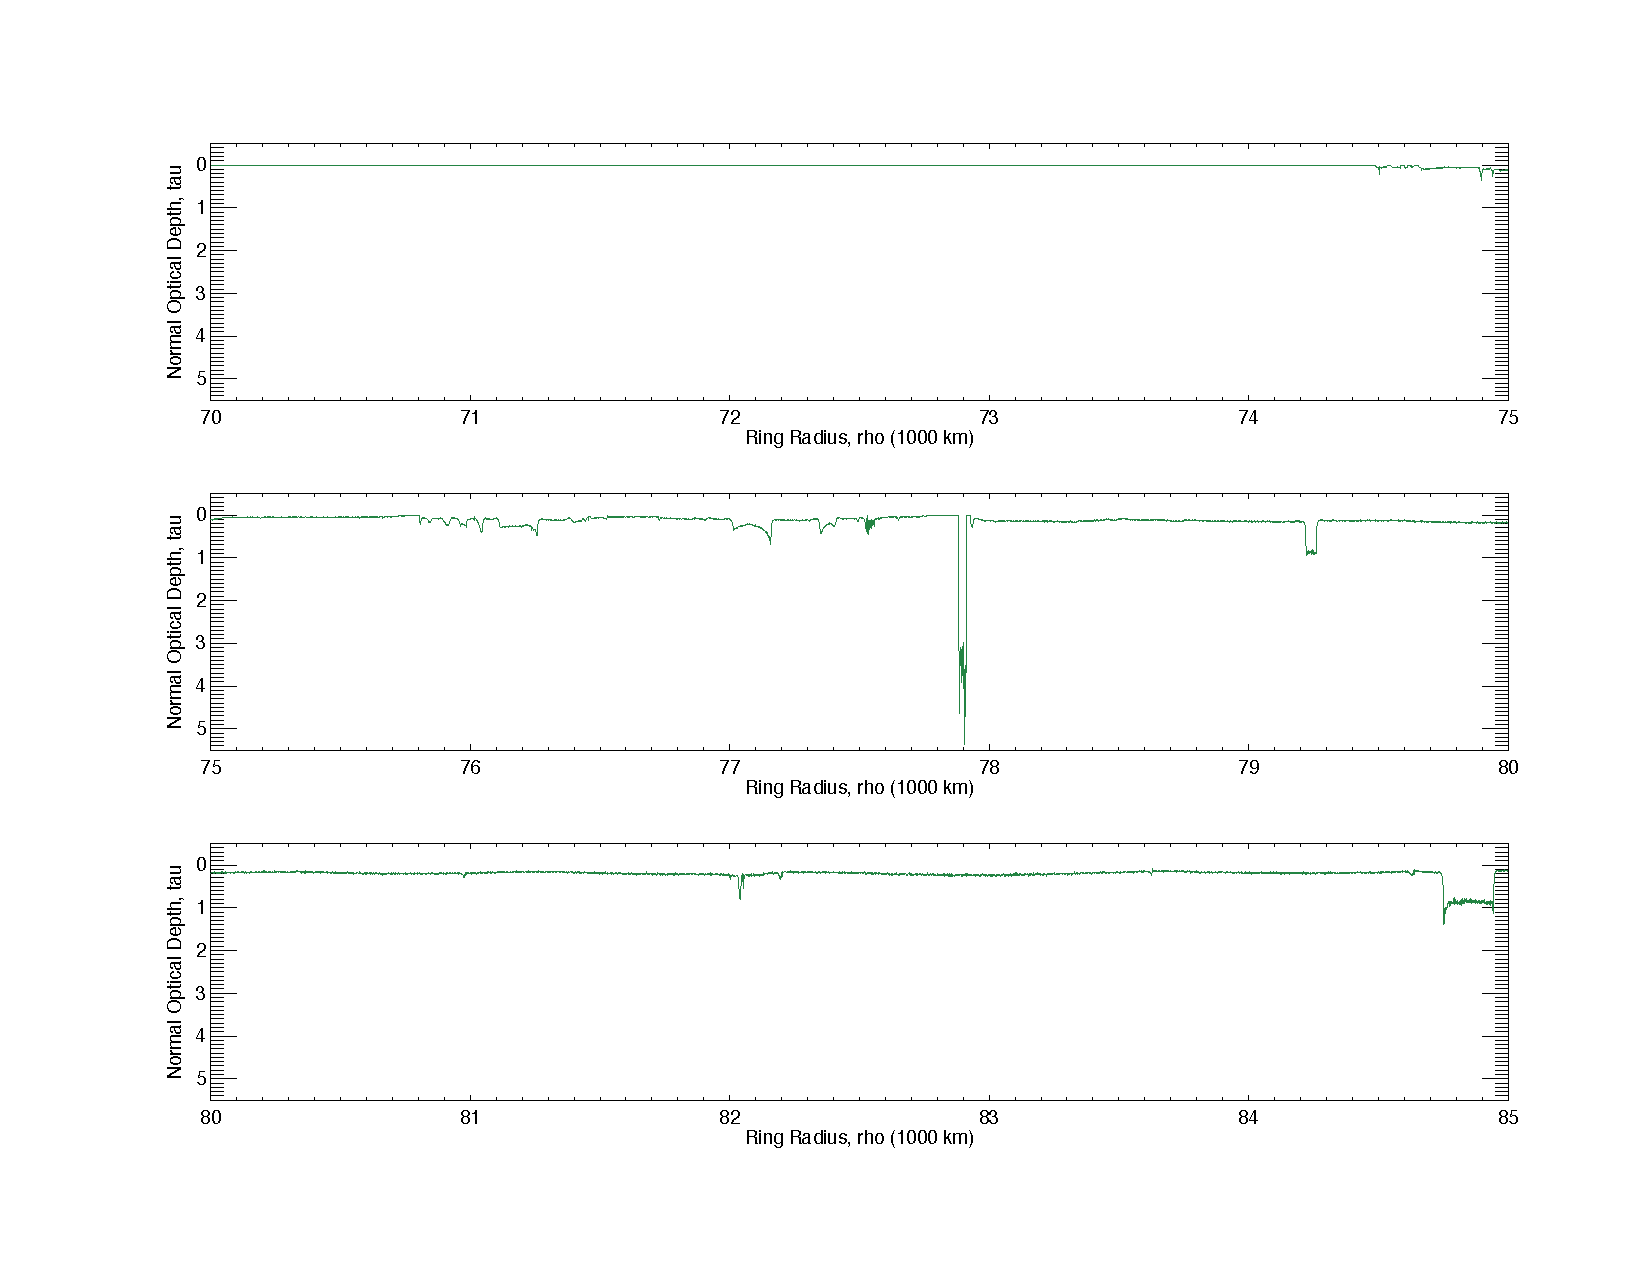
\includegraphics[page=1,width=\textwidth,trim = {1.1in 0.85in 0.8in 0.0in},clip]{Rev007_E_X43_summary_p2_08FEB2018.pdf}
    \caption[Normal Optical Depth Profiles from the Easy Data]{Rev7-E normal optical depth profiles reconstructed to remove diffraction effects at 1 and 10 km resolution (files RSS\_2005\_123\_X43\_E\_TAU\_01KM.tab and RSS\_2005\_123\_X43\_E\_TAU\_10KM.tab, respectively). The 1 km resolution profile is plotted in green and the 10 km resolution is plotted in blue. The dashed curves (black for the 1 km resolution profile and red for the 10 km resolution) identify the optical depth level at which the measurement SNR = 1, that is, the optical depth threshold $\tau_{TH}$.}
\end{figure}
\section{Example 2}
\begin{center}
    \LARGE{RSS\_2005\_123\_X43\_E \par
	Rev7-E Cassini Radio Science Ring Occultation: Geometry, Data Calibration, and Reconstructed Optical Depth and Phase Shift Profiles at 1 and 10km Resolution \par
	February 9, 2018\par}
\end{center}
\begin{figure}[H]
    \centering
    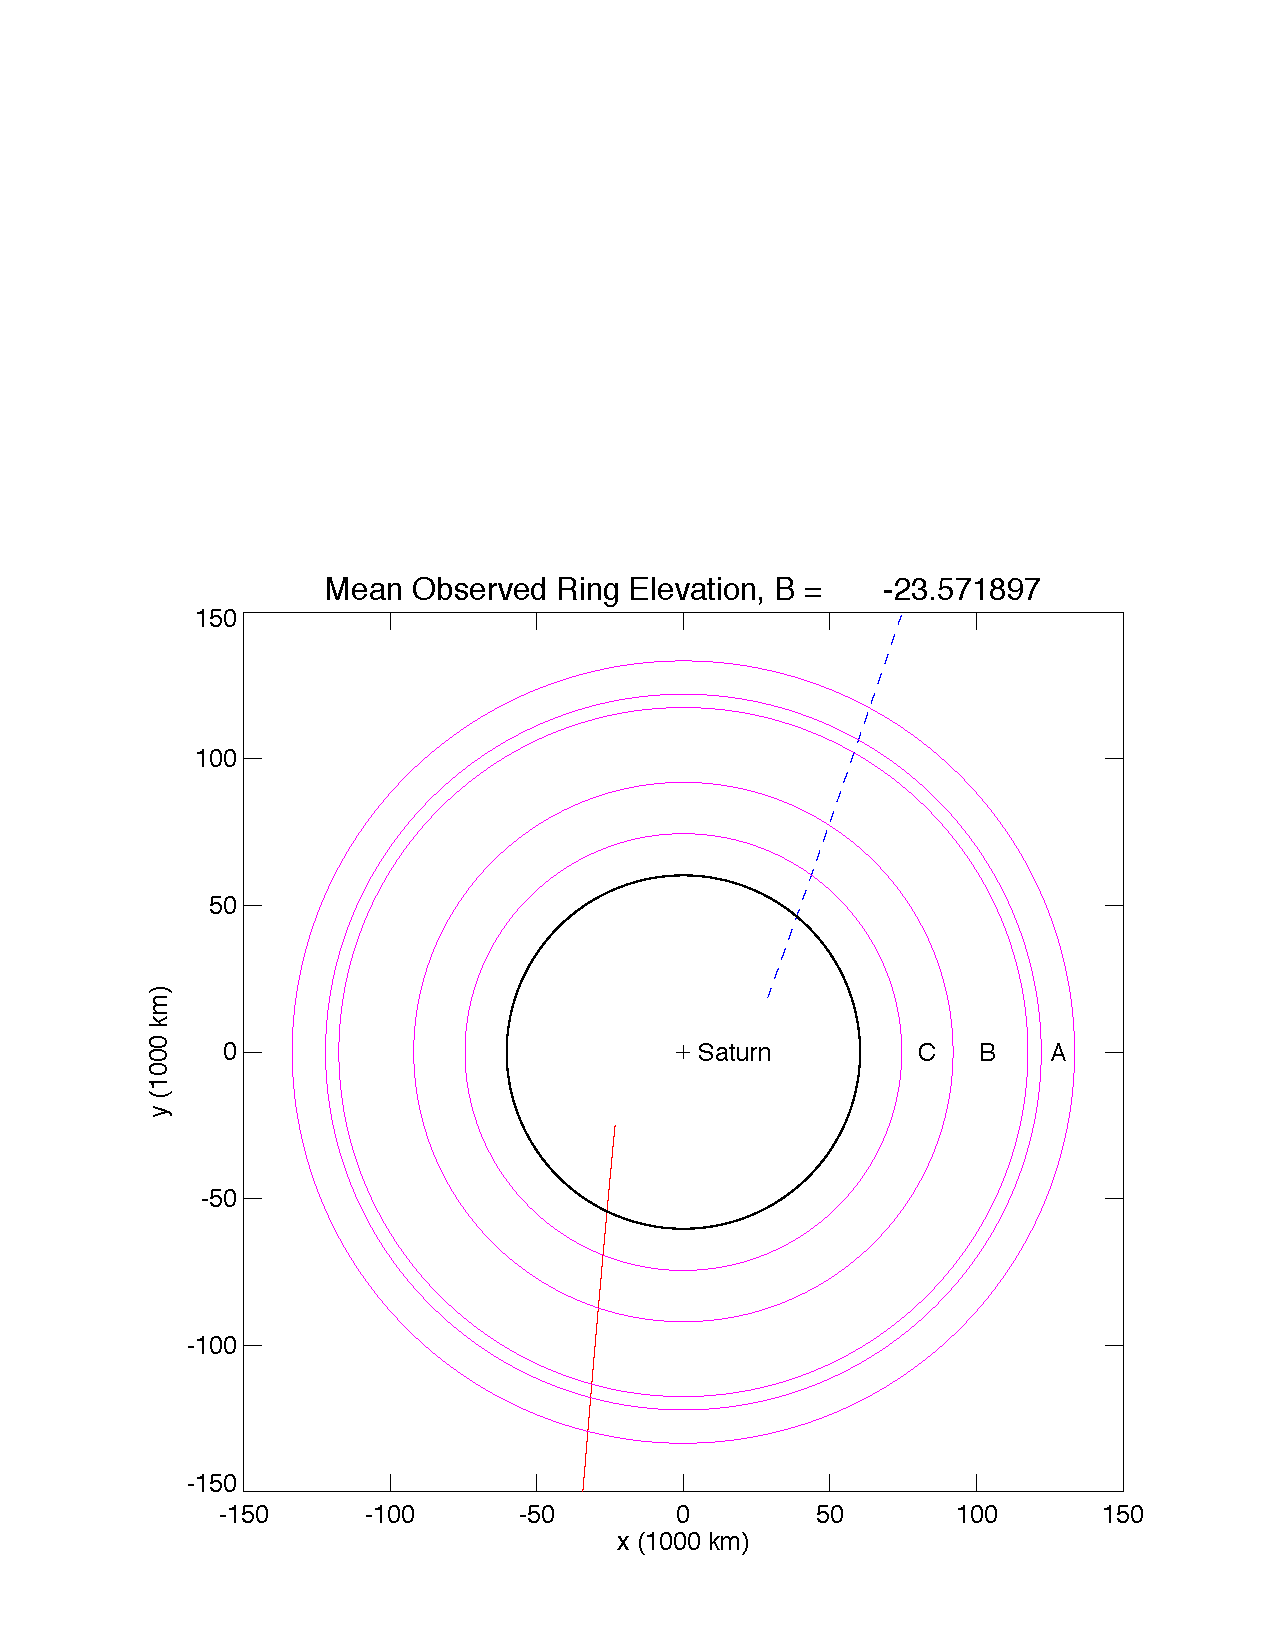
\includegraphics[page=1,trim = {0.67in 0.5in 0.5in 3.1in},clip,width=\textwidth]{Rev007_E_X43_summary_p1_08FEB2018.pdf}
    \caption[Radio Occultation Track]{The radio occultation track as seen looking down on the ring plane. The solid red track is relative to a reference direction defined by the direction to Earth, The dashed blue track is relative to a reference direction defined by the ascending node of J2000 on the ring plane.}
\end{figure}
\begin{table}[H]
    \centering
    \begin{tabular}{l l} 
        \hline
        Symbol 			& Parameter Name \\ % [0.5ex] 
        \hline
        $t_{OET}$		& OBSERVED EVENT TIME \\ 
        $t_{RET}$ 		& RING EVENT TIME \\
        $t_{SET}$ 		& SPACECRAFT EVENT TIME \\
        $\rho$	 		& RING RADIUS \\
        $\phi_{RL}$		& RING LONGITUDE \\
        $\phi_{ORA}$		& OBSERVED RING AZIMUTH \\
        $B$				& OBSERVED RING ELEVATION \\
        $D$				& SPACECRAFT TO RING INTERCEPT DISTANCE \\
        $\partial\rho/\partial t$	& RING INTERCEPT RADIAL VELOCITY \\
        $\partial\theta/\partial t$	& RING INTERCEPT AZIMUTHAL VELOCITY \\
        $F$				& FRESNEL SCALE \\
        $R_{impact}$		& IMPACT RADIUS \\
        $r_x$			& SPACECRAFT POSITION X \\
        $r_y$			& SPACECRAFT POSITION Y \\
        $r_z$			& SPACECRAFT POSITIION Z \\
        $v_x$			& SPACECRAFT VELOCITY X \\
        $v_y$			& SPACECRAFT VELOCITY Y \\
        $v_z$			& SPACECRAFT VELOCITY Z \\
        \hline
    \end{tabular}
    \caption[Glossary of Parameters from the Geo File]{Glossary of parameters in file RSS\_2005\_123\_X43\_E\_GEO.TAB. See companion label (.LBL) file for description of parameters.}
    \label{tab:easydata_glossary_of_geo_file}
\end{table}
\begin{table}[H]
    \centering
    \begin{tabular}{l l}
        \hline
        Symbol			& Parameter Name \\
        \hline
        $t_{OET}$			& OBSERVED EVENT TIME \\
        $f_{sky}$			& SKY FREQUENCY \\
        $f_{resid}$		& RESIDUAL FREQUENCY \\
        $P_{free}$		& FREESPACE POWER \\
        \hline
    \end{tabular}
    \caption[Glossary of Data from the Cal File]{Glossary of calibration data in file RSS\_2005\_123\_X43\_E\_CAL.TAB. See companion label (.LBL) file for description of the data.}
    \label{tab:easydata_glossary_from_cal_file}
\end{table}
\begin{table}[H]
    \centering
    \begin{tabular}{l l}
        \hline
        Symbol			& Parameter Name \\
        \hline
        $\rho$			& RING RADIUS \\
        $\Delta\rho$		& RADIUS CORRECTION \\
        $\phi_{RL}$		& RING LONGITUDE \\
        $\phi_{ORA}$		& OBSERVED RING AZIMUTH \\
        $\tau$			& NORMAL OPTICAL DEPTH \\
        $\phi$			& PHASE SHIFT \\
        $\tau_{TH}$		& NORMAL OPTICAL DEPTH THRESHOLD \\
        $t_{OET}$			& OBSERVED EVENT TIME \\
        $t_{RET}$			& RING EVENT TIME \\
        $t_{SET}$			& SPACECRAFT EVENT TIME \\
        $B$				& OBSERVED RING ELEVATION \\
        \hline
    \end{tabular}
    \caption[Glossary of Parameters in Tau File]{Glossary of optical depth, phase shift, and selected geometry parameters contained in files RSS\_2005\_123\_X43\_E\_TAU\_01KM.TAB and RSS\_2005\_123\_X43\_E\_TAU\_10KM.TAB. See companion label (.LBL) files for description of the data.}
    \label{tab:easydata_parameters_from_tau_file}
\end{table}
\begin{figure}[H]
    \centering
    \includegraphics[page=2,trim = {0.8in 0.5in 0.21in 0.45in},clip,width=\textwidth]{Rev007_E_X43_summary_p1_08FEB2018.pdf}
    \caption{Occultation geometry parameters in file RSS\_2005\_123\_X43\_E\_GEO.tab}
\end{figure}
\begin{figure}[H]
    \centering
    \includegraphics[page=3,trim = {0.8in 0.5in 0.21in 0.45in},clip,width=\textwidth]{Rev007_E_X43_summary_p1_08FEB2018.pdf}
    \caption{See caption of Figure 1a.}
\end{figure}
\begin{figure}[H]
    \centering
    \includegraphics[page=4,trim = {0.67in 0.5in 0.45in 0.5in},clip,width=\textwidth]{Rev007_E_X43_summary_p1_08FEB2018.pdf}
    \caption[Calibration Data from Cal File]{Calibration data in file Rev007\_E\_X43\_CAL.TAB. The frequency residuals data (the smooth curve, in the second panel) is used to steer the carrier signal to the middle of the recording bandwidth. The free-space power data (the smooth curve in the third panel) is used to normalize signal power measurements so that the corresponding optical depth has nearly zero value in the absence of rings. Least-square fitting techniques to frequency and power estimates of the direct signal (the green curves in the second and third panels, respectively) are used to compute the calibration data.}
\end{figure}
\begin{figure}[H]
    \centering
    \includegraphics[page=5,trim = {0.8in 0.5in 0.21in 0.45in},clip,width=\textwidth]{Rev007_E_X43_summary_p1_08FEB2018.pdf}
    \caption[Ring Radius Correction from Selected Occultation Geometry]{Ring radius correction and selected occultation geometry parameters contained in the file
RSS\_2005\_123\_X43\_E\_TAU\_01KM.TAB (solid green).}
\end{figure}
\begin{figure}[H]
    \centering
    \resizebox{\textwidth}{0.4\textheight}{
    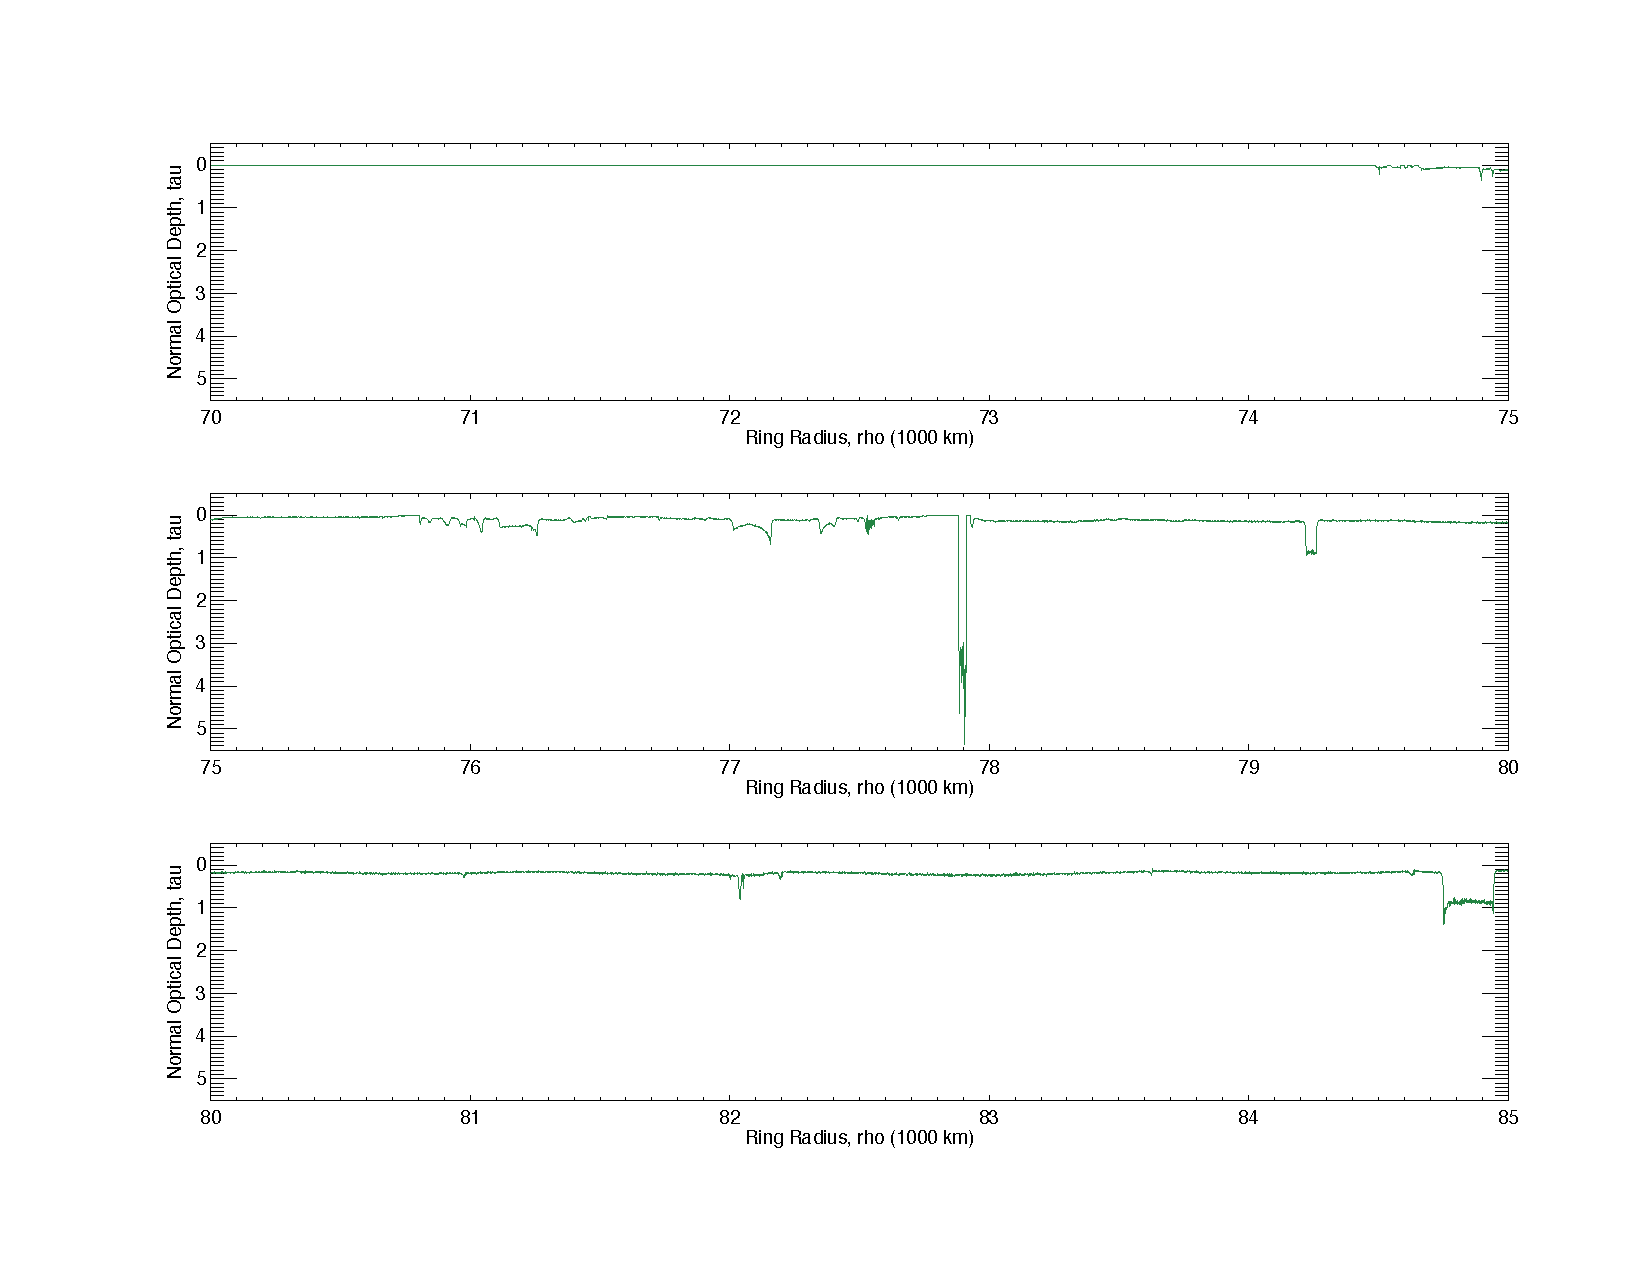
\includegraphics[page=1,width=\textwidth,trim = {1.1in 0.85in 0.8in 0.0in},clip]{Rev007_E_X43_summary_p2_08FEB2018.pdf}}
    \caption[Normal Optical Depth Profiles 70000-85000km]{Rev7-E normal optical depth profiles reconstructed to remove diffraction effects at 1 km resolution contained in the file RSS\_2005\_123\_X43\_E\_TAU\_01KM.tab. The 1 km resolution profile is plotted in green.}
\end{figure}
\begin{figure}[H]
    \centering
    \resizebox{\textwidth}{0.4\textheight}{
    \includegraphics[page=2,width=\textwidth,trim = {1.1in 0.85in 0.8in 0.0in},clip]{Rev007_E_X43_summary_p2_08FEB2018.pdf}}
    \caption[Normal Optical Depth Profiles 85000-100000km]{Rev7-E normal optical depth profiles reconstructed to remove diffraction effects at 1 km resolution contained in the file RSS\_2005\_123\_X43\_E\_TAU\_01KM.tab. The 1 km resolution profile is plotted in green.}
\end{figure}
\begin{figure}[H]
    \centering
    \resizebox{\textwidth}{0.4\textheight}{
    \includegraphics[page=3,width=\textwidth,trim = {1.1in 0.85in 0.8in 0.0in},clip]{Rev007_E_X43_summary_p2_08FEB2018.pdf}}
    \caption[Normal Optical Depth Profiles 100000-115000km]{Rev7-E normal optical depth profiles reconstructed to remove diffraction effects at 1 km resolution contained in the file RSS\_2005\_123\_X43\_E\_TAU\_01KM.tab. The 1 km resolution profile is plotted in green.}
\end{figure}
\begin{figure}[H]
    \centering
    \resizebox{\textwidth}{0.4\textheight}{
    \includegraphics[page=4,width=\textwidth,trim = {1.1in 0.85in 0.8in 0.0in},clip]{Rev007_E_X43_summary_p2_08FEB2018.pdf}}
    \caption[Normal Optical Depth Profiles 115000-130000km]{Rev7-E normal optical depth profiles reconstructed to remove diffraction effects at 1 km resolution (file RSS\_2005\_123\_X43\_E\_TAU\_01KM.tab). The 1 km resolution profile is plotted in green.}
\end{figure}
\begin{figure}[H]
    \centering
    \resizebox{\textwidth}{0.4\textheight}{
    \includegraphics[page=5,width=\textwidth,trim = {1.1in 0.85in 0.8in 0.0in},clip]{Rev007_E_X43_summary_p2_08FEB2018.pdf}}
    \caption[Normal Optical Depth Profiles 130000-145000km]{Rev7-E normal optical depth profiles reconstructed to remove diffraction effects at 1 km resolution contained in the file RSS\_2005\_123\_X43\_E\_TAU\_01KM.tab. The 1 km resolution profile is plotted in green.}
\end{figure}
\begin{figure}[H]
    \centering
    \resizebox{\textwidth}{0.4\textheight}{
    \includegraphics[page=6,width=\textwidth,trim = {1.1in 0.85in 0.8in 0.0in},clip]{Rev007_E_X43_summary_p2_08FEB2018.pdf}}
    \caption[Phase Shift Profile]{Rev7-E Phase shift profile reconstructed to remove diffraction effects at 1 km resolution contained in the file RSS\_2005\_123\_X43\_E\_TAU\_01KM.TAB. The 1 km resolution profile is plotted in solid green.}
\end{figure}
\end{document}